\documentclass{beamer}
\usetheme{Berlin}
%\usecolortheme{dolphin}
\usepackage[utf8]{inputenc}
\usepackage[T1]{fontenc}


\usepackage{csvsimple}
\usepackage{graphicx}
\graphicspath{ {./files/} } % Path relative to the main .tex file 
\newcommand{\fg}[2]{%
  \begin{center}
      \includegraphics[width = #1\textwidth]{#2}%
  \end{center}
}


\usepackage{verbatim}






\title{Regressione Lineare e Anova}

\subtitle{Progetto di Inferenza Statistica}

\author{T. Bucci, G. Corbo, D. Fabroni}

\institute{Politecnico di Milano}

\date{Luglio 2021}





\begin{document}

\frame{\titlepage}

\begin{frame}
    \frametitle{Table of Contents}
    \tableofcontents
\end{frame}

\section{Presentazione del dataset}
\begin{frame}
    \frametitle{Scelta del dataset: Biomechanical features of orthopedic patients}
    Fonte: Lichman, M. (2013). UCI Machine Learning Repository [\texttt{http://archive.ics.uci.edu/ml}]. Irvine, CA: University of California, School of Information and Computer Science
    %\footnote{\texttt{https://www.kaggle.com/uciml/biomechanical-features-of-orthopedic-patients?select=column_3C_weka.csv}}
\end{frame}


\begin{frame}
    \frametitle{Covariate presenti}
    \begin{itemize}
        \item pelvic incidence (continua)
        \item pelvic tilt (continua)
        \item lumbar lordosis angle (continua)
        \item sacral slope (continua)
        \item pelvic radius (continua)
        \item grade of spondylolisthesis (continua)
        \item class (categorica)
    \end{itemize}
    con $310$ osservazioni.
\end{frame}


\begin{frame}
	Sono indici dell'inclinazione del bacino sul piano sagittale.
	\fg{0.5}{piani.png}
	Le classi sono \emph{Hernia, Spondylolisthesis, Normal}. % Una non esclude l'altra in realtà
\end{frame}


\begin{frame}
    \begin{center}
        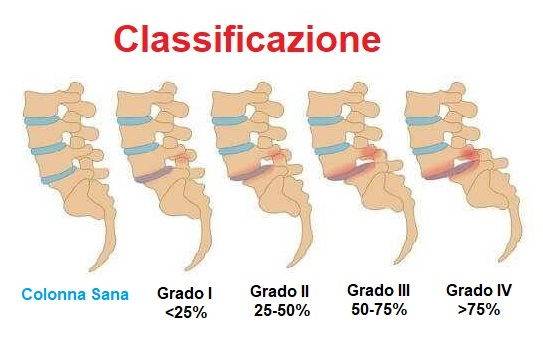
\includegraphics[width=0.9\textwidth]{classificazione-spondilolistesi.jpg}
    \end{center}
\end{frame}


\section{Obiettivo}
\begin{frame}
    Vogliamo fare una regressione su misurazioni fisiche della zona pelvica...
    \begin{center}
        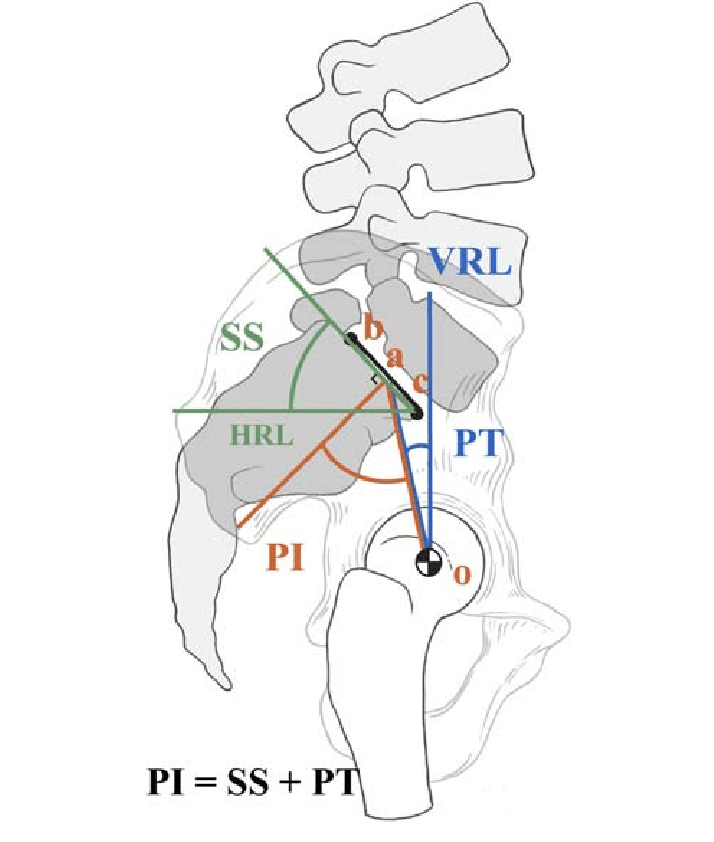
\includegraphics[width=0.35\textwidth]{bacino.png}
    \end{center}
\end{frame}


\begin{frame}
    ... per poter stimare il \textbf{lumbar lordosis angle}, un parametro che riguarda la sezione medio-bassa della schiena che misura la concavità della zona lombare della schiena.
    \begin{center}
        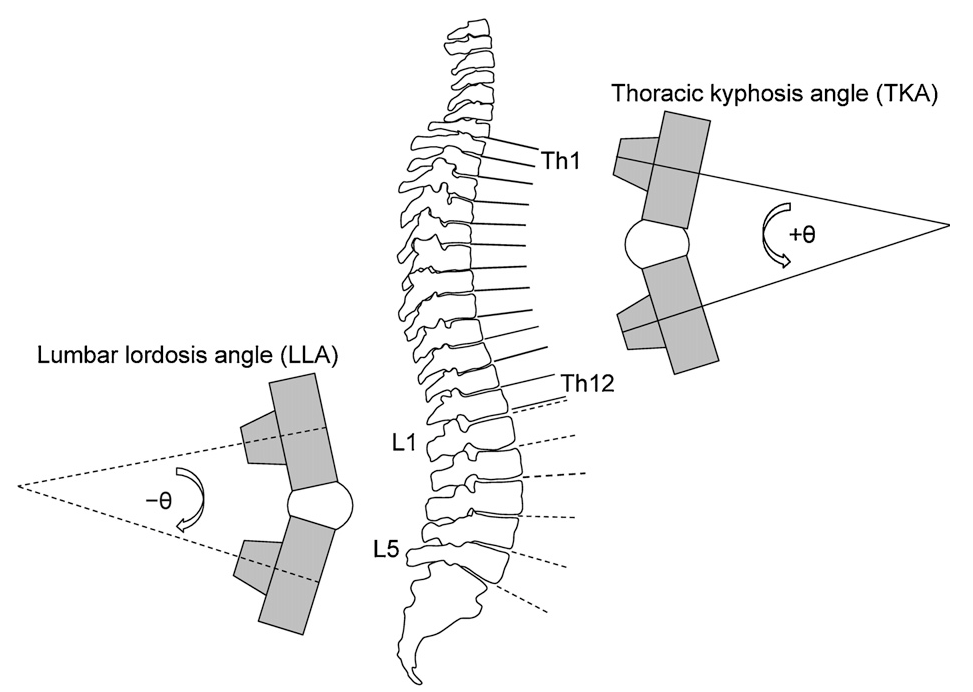
\includegraphics[width=0.5\textwidth]{lla.png}
    \end{center}
\end{frame}


\begin{frame}
    Vantaggi di questo approccio
    \begin{itemize}
        \item Poter prevedere una caratteristica della schiena senza fare una radiografia completa della schiena
        \item Risparmio di costi della radiografia
        \item Riduzione della quantità di raggi X a cui il paziente è esposto
    \end{itemize}
\end{frame}

\section{Modello lineare}
\begin{frame}[fragile]
\frametitle{Overview dei dati}
\tiny
	\begin{verbatim}
  pelvic_incidence pelvic_tilt lumbar_lordosis_angle sacral_slope pelvic_radius
1         63.02782   22.552586              39.60912     40.47523      98.67292
2         39.05695   10.060991              25.01538     28.99596     114.40543
3         68.83202   22.218482              50.09219     46.61354     105.98514
4         69.29701   24.652878              44.31124     44.64413     101.86850
5         49.71286    9.652075              28.31741     40.06078     108.16872
6         40.25020   13.921907              25.12495     26.32829     130.32787
  degree_spondylolisthesis  class
1                -0.254400 Hernia
2                 4.564259 Hernia
3                -3.530317 Hernia
4                11.211523 Hernia
5                 7.918501 Hernia
6                 2.230652 Hernia
	\end{verbatim}

	{\normalsize Non ci sono degli NA.}
\end{frame}



\begin{frame}
	\fg{1}{00ggpairs}
\end{frame}



\begin{frame}[fragile]
	Generiamo il primo modello lineare, come risposta \texttt{lumbar\_lordosis\_angle}.
	
	Escludiamo \texttt{class}, che è la categorica.

	{\tiny
	\begin{verbatim}
		Call:
		lm(formula = lumbar_lordosis_angle ~ . - class, data = biomech)

		Residuals:
		    Min      1Q  Median      3Q     Max 
		-76.720  -7.415  -1.261   6.878  70.183 

		Coefficients: (1 not defined because of singularities)
		                          Estimate Std. Error t value Pr(>|t|)    
		(Intercept)              -10.55489    8.59928  -1.227   0.2206    
		pelvic_incidence           0.76884    0.06996  10.989   <2e-16 ***
		pelvic_tilt               -0.11410    0.09650  -1.182   0.2380    
		sacral_slope                    NA         NA      NA       NA    
		pelvic_radius              0.14092    0.05911   2.384   0.0177 *  
		degree_spondylolisthesis   0.05166    0.02555   2.022   0.0441 *  
		---
		Signif. codes:  0 ‘***’ 0.001 ‘**’ 0.01 ‘*’ 0.05 ‘.’ 0.1 ‘ ’ 1

		Residual standard error: 12.76 on 305 degrees of freedom
		Multiple R-squared:  0.5334,	Adjusted R-squared:  0.5272 
		F-statistic: 87.15 on 4 and 305 DF,  p-value: < 2.2e-16

	\end{verbatim}
	}
\end{frame}


\begin{frame}
	$R^2_{adj}$ iniziale abbastanza buono come punto di partenza: $0.5272$.

	Molto significativo \texttt{pelvic\_incidence}.

	p-value dell'F-test 2.2e-16, c'è evidenza per dire che almeno una covariata sia significativa.

	Ci sono NA in corrispondenza di \texttt{sacral\_slope}, scopriamo che è indice di lineare dipendenza da altre covariate, procediamo quindi subito con l'analisi di questo aspetto.
\end{frame}

\begin{frame}[fragile]
	Prevediamo \texttt{sacral\_slope} in funzione di tutto il resto, tranne la risposta originale e la categorica.

	{\tiny
	\begin{verbatim}
		Call:
lm(formula = sacral_slope ~ . - class - lumbar_lordosis_angle, 
    data = biomech)

Residuals:
       Min         1Q     Median         3Q        Max 
-1.091e-08 -5.072e-10  1.020e-10  3.703e-10  1.057e-08 

Coefficients:
                           Estimate Std. Error    t value Pr(>|t|)    
(Intercept)               6.414e-10  3.159e-09  2.030e-01    0.839    
pelvic_incidence          1.000e+00  2.570e-11  3.891e+10   <2e-16 ***
pelvic_tilt              -1.000e+00  3.545e-11 -2.821e+10   <2e-16 ***
pelvic_radius            -8.878e-12  2.171e-11 -4.090e-01    0.683    
degree_spondylolisthesis  4.338e-12  9.388e-12  4.620e-01    0.644    
---
Signif. codes:  0 ‘***’ 0.001 ‘**’ 0.01 ‘*’ 0.05 ‘.’ 0.1 ‘ ’ 1

Residual standard error: 4.687e-09 on 305 degrees of freedom
Multiple R-squared:      1,	Adjusted R-squared:      1 
F-statistic: 6.337e+20 on 4 and 305 DF,  p-value: < 2.2e-16
	\end{verbatim}
	}
\end{frame}


\begin{frame}
	$R^{2}_{adj}$ vale $1$, osservando i $\beta$ scopriamo che
	$$ \text{sacralslope} + \text{pelvictilt} = \text{pelvicincidence}$$
	In ambito medico abbiamo conferma di questa cosa:

	\textit{Pelvic tilt and sacral slope are two angles directly correlated with the pelvic incidence angle. The angle of incidence is the algebraic sum of two angles: pelvic tilt (PT) and sacral slope (SS)}\footnote{https://www.ncbi.nlm.nih.gov/pmc/articles/PMC3175921/}

	Escludiamo questa covariata.
\end{frame}





%\begin{frame}
%	Vediamo anche la correlazione.
%	\fg{0.6}{01coorplot}
%\end{frame}






\begin{frame}[fragile]
	Procediamo con il nostro modello escludendo la \texttt{sacral\_slope} e la categorica.

	{\tiny
	\begin{verbatim}
		Call:
lm(formula = lumbar_lordosis_angle ~ . - class - sacral_slope, 
    data = biomech)

Residuals:
    Min      1Q  Median      3Q     Max 
-76.720  -7.415  -1.261   6.878  70.183 

Coefficients:
                          Estimate Std. Error t value Pr(>|t|)    
(Intercept)              -10.55489    8.59928  -1.227   0.2206    
pelvic_incidence           0.76884    0.06996  10.989   <2e-16 ***
pelvic_tilt               -0.11410    0.09650  -1.182   0.2380    
pelvic_radius              0.14092    0.05911   2.384   0.0177 *  
degree_spondylolisthesis   0.05166    0.02555   2.022   0.0441 *  
---
Signif. codes:  0 ‘***’ 0.001 ‘**’ 0.01 ‘*’ 0.05 ‘.’ 0.1 ‘ ’ 1

Residual standard error: 12.76 on 305 degrees of freedom
Multiple R-squared:  0.5334,	Adjusted R-squared:  0.5272 
F-statistic: 87.15 on 4 and 305 DF,  p-value: < 2.2e-16
	\end{verbatim}
	}
\end{frame}





\begin{frame}
	\frametitle{Controlliamo le ipotesi}
	L'omoschedasticità non è fantastica e lo Shapiro test rifiuta la normalità con un p-value di 3.878e-11.
	\begin{figure}
	   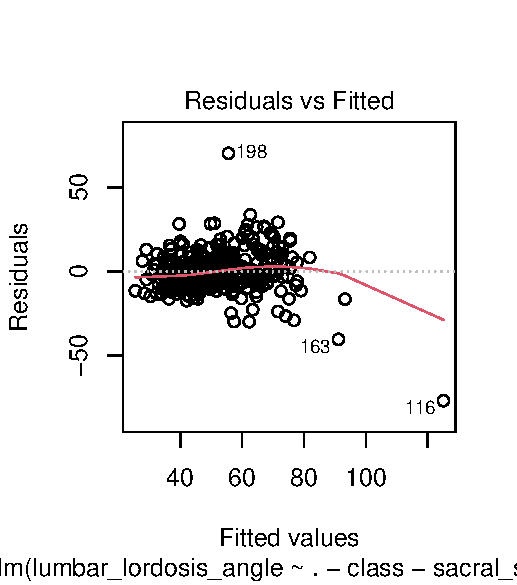
\includegraphics[width=0.475\textwidth]{02omoschedasticita}
	   \hfill
	   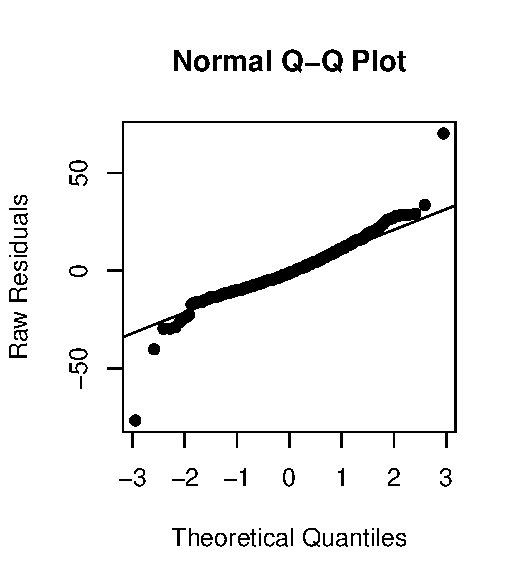
\includegraphics[width=0.475\textwidth]{03qqplot}
	\end{figure}
\end{frame}




\begin{frame}[fragile]
	Procediamo dapprima con la pulizia del dataset, controllando se migliorano le ipotesi di lavoro, e nel caso procediamo con la trasformazione box cox.
	
	\vspace*{1cm}
	I \textbf{punti leva} ($h_{ii}>2p/n$) risultano:

	\begin{verbatim}
		 10  52  76  84  86  96 116 123 142 163
		164 168 174 180 181 191 193 198 203 207
	\end{verbatim}

	\vspace*{1cm}
	Vediamo anche residui studentizzati e standardizzati.
\end{frame}



\begin{frame}[fragile]
	Gli standardizzati sono
	\begin{verbatim}
 52  72  75  83  94  99 113 116
125 135 143 163 183 198 202 203
	\end{verbatim}
	e coincidono con gli studentizzati.
\end{frame}


\begin{frame}
	\fg{0.6}{05graficone}
\end{frame}




\begin{frame}
	\textbf{Punti influenti}
	\fg{0.6}{06influencialPlot}
\end{frame}



\begin{frame}[fragile]
	Dopo aver tolto i leverage:

	{\tiny
	\begin{verbatim}
		Call:
lm(formula = lumbar_lordosis_angle ~ . - class - sacral_slope, 
    data = biomech, subset = (lev < 2 * p/n))

Residuals:
    Min      1Q  Median      3Q     Max 
-38.740  -6.327  -0.724   5.792  26.955 

Coefficients:
                          Estimate Std. Error t value Pr(>|t|)    
(Intercept)              -14.65892    7.78281  -1.884  0.06065 .  
pelvic_incidence           0.82717    0.06289  13.152  < 2e-16 ***
pelvic_tilt               -0.37281    0.09005  -4.140 4.58e-05 ***
pelvic_radius              0.15686    0.05499   2.853  0.00465 ** 
degree_spondylolisthesis   0.20055    0.03096   6.477 4.08e-10 ***
---
Signif. codes:  0 ‘***’ 0.001 ‘**’ 0.01 ‘*’ 0.05 ‘.’ 0.1 ‘ ’ 1

Residual standard error: 10.12 on 285 degrees of freedom
Multiple R-squared:  0.6929,	Adjusted R-squared:  0.6886 
F-statistic: 160.7 on 4 and 285 DF,  p-value: < 2.2e-16
	\end{verbatim}
	}
\end{frame}



\begin{frame}[fragile]
	Dopo aver tolto gli studentizzati:

	{\tiny
	\begin{verbatim}
Call:
lm(formula = lumbar_lordosis_angle ~ . - class - sacral_slope, 
    data = biomech, subset = (abs(stud) < 2))

Residuals:
     Min       1Q   Median       3Q      Max 
-24.7494  -6.7045  -0.8731   6.1216  25.1839 

Coefficients:
                         Estimate Std. Error t value Pr(>|t|)    
(Intercept)              -7.11477    6.20910  -1.146   0.2528    
pelvic_incidence          0.87282    0.05160  16.914  < 2e-16 ***
pelvic_tilt              -0.39784    0.07492  -5.310 2.19e-07 ***
pelvic_radius             0.08100    0.04293   1.887   0.0602 .  
degree_spondylolisthesis  0.13697    0.02437   5.621 4.48e-08 ***
---
Signif. codes:  0 ‘***’ 0.001 ‘**’ 0.01 ‘*’ 0.05 ‘.’ 0.1 ‘ ’ 1

Residual standard error: 9.021 on 289 degrees of freedom
Multiple R-squared:  0.7298,	Adjusted R-squared:  0.7261 
F-statistic: 195.2 on 4 and 289 DF,  p-value: < 2.2e-16
	\end{verbatim}
	}
\end{frame}





\begin{frame}[fragile]
	Dopo aver tolto i leverage e gli studentizzati:

	{\tiny
	\begin{verbatim}
Call:
lm(formula = lumbar_lordosis_angle ~ . - class - sacral_slope, 
    data = biomech, subset = (abs(stud) < 2 | lev < 2 * p/n))

Residuals:
    Min      1Q  Median      3Q     Max 
-34.290  -7.025  -0.731   5.986  31.766 

Coefficients:
                         Estimate Std. Error t value Pr(>|t|)    
(Intercept)              -6.11635    6.98922  -0.875   0.3822    
pelvic_incidence          0.83386    0.05816  14.337  < 2e-16 ***
pelvic_tilt              -0.40375    0.08410  -4.801 2.50e-06 ***
pelvic_radius             0.09063    0.04823   1.879   0.0612 .  
degree_spondylolisthesis  0.16506    0.02716   6.077 3.71e-09 ***
---
Signif. codes:  0 ‘***’ 0.001 ‘**’ 0.01 ‘*’ 0.05 ‘.’ 0.1 ‘ ’ 1

Residual standard error: 10.32 on 300 degrees of freedom
Multiple R-squared:  0.6759,	Adjusted R-squared:  0.6716 
F-statistic: 156.4 on 4 and 300 DF,  p-value: < 2.2e-16
	\end{verbatim}
	}
\end{frame}



\begin{frame}[fragile]
	Aggiungiamo il calcolo dell'AIC.
	\begin{verbatim}
> AIC(g_post_lev)
[1] 2172.373
> AIC(g_post_rs)
[1] 2134.629
> AIC(g_post_both)
[1] 2296.307
	\end{verbatim}

	Il modello migliore è quello senza i punti influenti trovati coi residui studentizzati, avendo $R^{2}_{adj}$ maggiore e AIC minore.

	L'$R^2_{adj}$ aumenta notevolmente a 0.7261.

	p-value è 2.2e-16, ci sono ancora covariate non significative, stavolta diverse da prima.
\end{frame}



\begin{frame}
	\fg{0.6}{04residuistudentizzati}
\end{frame}



\begin{frame}
	L'omoschedasticità migliora, lo Shapiro test rifiuta la normalità con un p-value di 0.04041.
	\begin{figure}
	   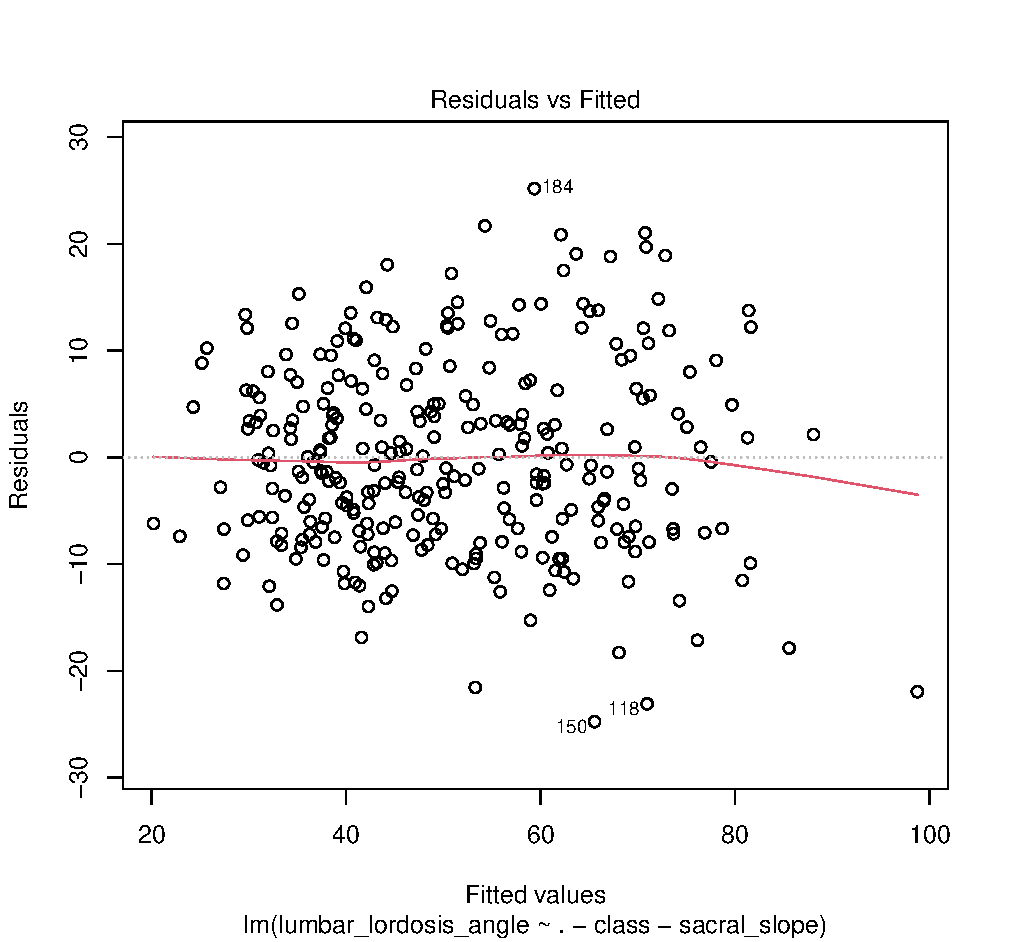
\includegraphics[width=0.475\textwidth]{07omoschedasticita}
	   \hfill
	   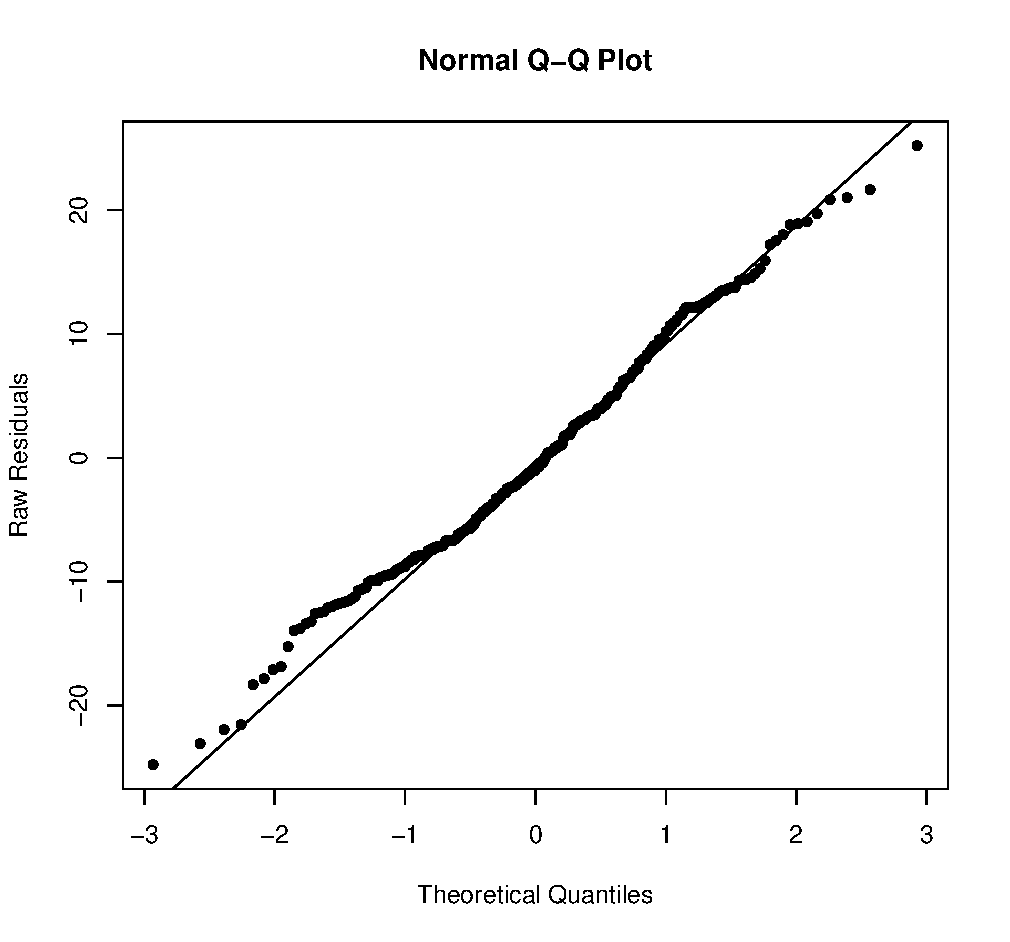
\includegraphics[width=0.475\textwidth]{08qqplot}
	\end{figure}
\end{frame}


\begin{frame}
	\frametitle{Trasformazione box cox}
	Otteniamo $\lambda = 0.6262626$
	\fg{0.6}{09boxcox}
\end{frame}




\begin{frame}[fragile]
	Generiamo il nuovo ML dove modelliamo $\frac{Y^{\lambda}-1}{\lambda}$

	{\tiny
	\begin{verbatim}
		Call:
lm(formula = (lumbar_lordosis_angle^best_lambdagl - 1)/best_lambdagl ~ 
    . - class - sacral_slope, data = biomech, subset = (abs(stud) < 
    2))

Residuals:
    Min      1Q  Median      3Q     Max 
-5.5750 -1.5905 -0.1978  1.4263  5.4229 

Coefficients:
                          Estimate Std. Error t value Pr(>|t|)    
(Intercept)               3.517005   1.436634   2.448   0.0150 *  
pelvic_incidence          0.204373   0.011940  17.117  < 2e-16 ***
pelvic_tilt              -0.096457   0.017334  -5.565 6.00e-08 ***
pelvic_radius             0.017717   0.009934   1.784   0.0755 .  
degree_spondylolisthesis  0.030430   0.005638   5.397 1.41e-07 ***
---
Signif. codes:  0 ‘***’ 0.001 ‘**’ 0.01 ‘*’ 0.05 ‘.’ 0.1 ‘ ’ 1

Residual standard error: 2.087 on 289 degrees of freedom
Multiple R-squared:  0.7288,	Adjusted R-squared:  0.725 
F-statistic: 194.1 on 4 and 289 DF,  p-value: < 2.2e-16
	\end{verbatim}
	}

\end{frame}


\begin{frame}
	$R^2_{adj}$ diminuisce da 0.7261 a 0.725.

	Verifichiamo se ora le ipotesi di normalità sono soddisfatte.
\end{frame}

\begin{frame}
	L'omoschedasticità rimane la stessa, lo Shapiro test non rifiuta la normalità con un p-value di 0.196.
	\begin{figure}
	   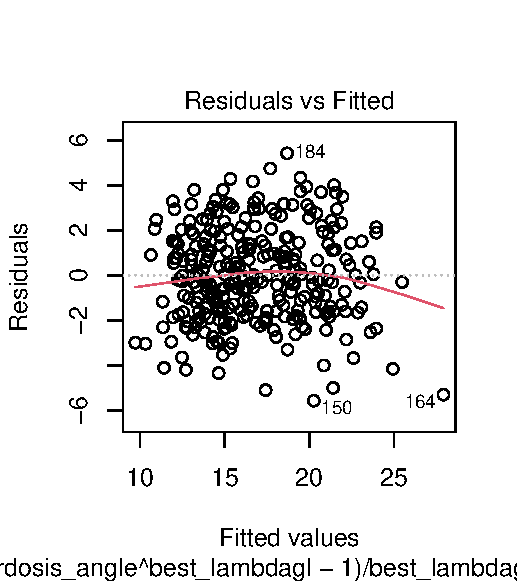
\includegraphics[width=0.475\textwidth]{10omoschedasticita}
	   \hfill
	   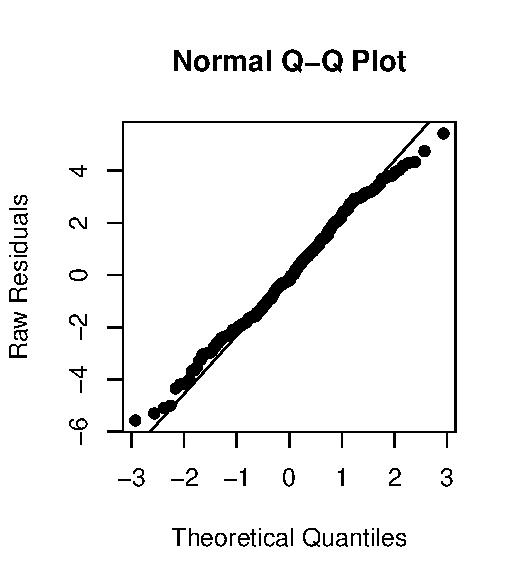
\includegraphics[width=0.475\textwidth]{11qqplot}
	\end{figure}
\end{frame}




\begin{frame}[fragile]
\frametitle{Selezione delle covariate}
	Rimuoviamo \texttt{pelvic\_radius} che ha un p-value \textit{one-at-a-time} di 0.0755, c'è evidenza per dire che non è significativo.

	{\tiny
	\begin{verbatim}
		Call:
lm(formula = (lumbar_lordosis_angle^best_lambdagl - 1)/best_lambdagl ~ 
    . - class - sacral_slope - pelvic_radius, data = biomech, 
    subset = (abs(stud) < 2))

Residuals:
    Min      1Q  Median      3Q     Max 
-5.8320 -1.6205 -0.0449  1.4739  5.4439 

Coefficients:
                          Estimate Std. Error t value Pr(>|t|)    
(Intercept)               5.902680   0.526115  11.219  < 2e-16 ***
pelvic_incidence          0.196926   0.011228  17.539  < 2e-16 ***
pelvic_tilt              -0.089619   0.016969  -5.282 2.52e-07 ***
degree_spondylolisthesis  0.031657   0.005617   5.635 4.13e-08 ***
---
Signif. codes:  0 ‘***’ 0.001 ‘**’ 0.01 ‘*’ 0.05 ‘.’ 0.1 ‘ ’ 1

Residual standard error: 2.095 on 290 degrees of freedom
Multiple R-squared:  0.7258,	Adjusted R-squared:  0.723 
F-statistic: 255.9 on 3 and 290 DF,  p-value: < 2.2e-16
	\end{verbatim}
	}
\end{frame}



\begin{frame}
	$R^2_{adj}$ scende da 0.725 a 0.723, ma semplifica di molto il modello, quindi procediamo con questa modifica.

	Verifichiamo come cambiano le ipotesi di normalità e omoschedasticità.
\end{frame}


\begin{frame}
	L'omoschedasticità rimane la stessa, lo Shapiro test migliora con un p-value di 0.22.
	\begin{figure}
	   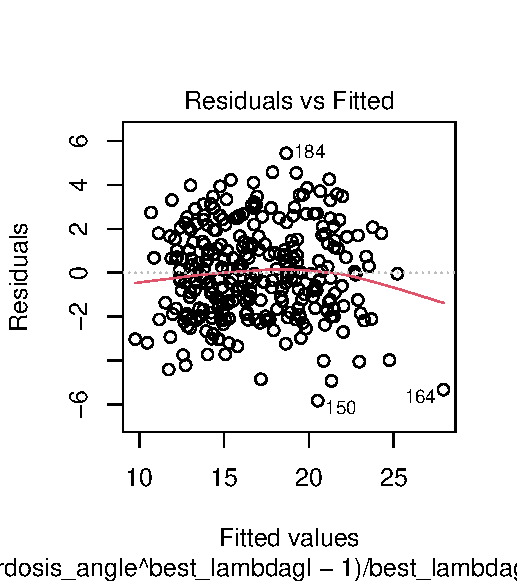
\includegraphics[width=0.475\textwidth]{12omoschedasticita}
	   \hfill
	   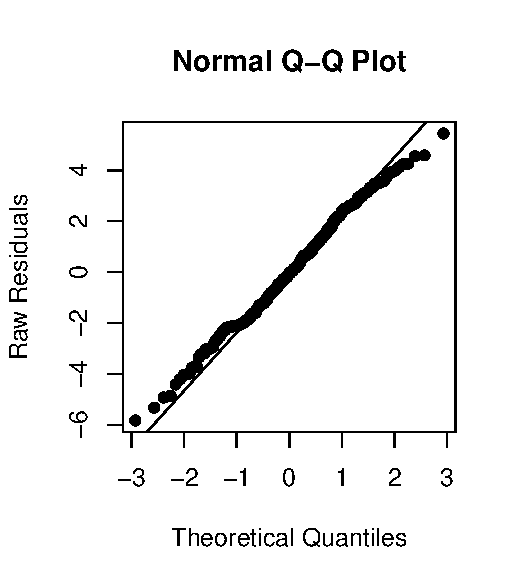
\includegraphics[width=0.475\textwidth]{13qqplot}
	\end{figure}
\end{frame}

\begin{frame}
	\frametitle{Modello conclusivo}
	$$
	\frac{LLA^{\lambda}-1}{\lambda} = 5.902680 + 0.196926 \cdot \text{PI} -0.089619 \cdot \text{PT} + 0.031657 \cdot \text{DS}
	$$
	dove $\lambda=0.6262626$.
\end{frame}






\section{ANOVA}

\begin{frame}
	Procediamo ora con l'ANOVA, siamo interessati a capire se la media della nostra risposta LLA è diversa tra le classi.
	\fg{0.6}{14boxplot}
\end{frame}

\begin{frame}[fragile]
	Lo Shapiro test ci porta tuttavia a rifiutare la normalità nei gruppi.
	\begin{verbatim}
		           Hernia            Normal Spondylolisthesis 
       0.68493698        0.01650640        0.07089939
	\end{verbatim}

	Sia il Levene test che il Bartlett test ci portano a rifiutare anche l'omoschedasticità tra i gruppi.
	{\tiny
	\begin{verbatim}
		> leveneTest(biomech$lumbar_lordosis_angle, biomech$class)
Levene's Test for Homogeneity of Variance (center = median)
       Df F value    Pr(>F)    
group   2  9.8185 7.357e-05 ***
      307                      
---
> bartlett.test(biomech$lumbar_lordosis_angle, biomech$class)

	Bartlett test of homogeneity of variances

data:  biomech$lumbar_lordosis_angle and biomech$class
Bartlett's K-squared = 23.183, df = 2, p-value = 9.242e-06
	\end{verbatim}
	}
\end{frame}



\begin{frame}
	\frametitle{Trasformazione box cox}
	Otteniamo $\lambda = 0.31$
	\fg{0.6}{15boxcox}
\end{frame}




\begin{frame}[fragile]
	Lo Shapiro test ci porta ora a non rifiutare la normalità nei gruppi.
	\begin{verbatim}
           Hernia            Normal Spondylolisthesis 
        0.1834879         0.9761894         0.7439135 
	\end{verbatim}

	Sia il Levene test che il Bartlett test ora confermano l'omoschedasticità.
	{\tiny
	\begin{verbatim}
		> leveneTest( (biomech$lumbar_lordosis_angle^best_lambda -1)/best_lambda ,biomech$class )
Levene's Test for Homogeneity of Variance (center = median)
       Df F value Pr(>F)
group   2  0.5628 0.5702
      307                   
---
> bartlett.test(  (biomech$lumbar_lordosis_angle^best_lambda -1)/best_lambda ,biomech$class )

	Bartlett test of homogeneity of variances

data:  (biomech$lumbar_lordosis_angle^best_lambda - 1)/best_lambda and biomech$class
Bartlett's K-squared = 0.49971, df = 2, p-value = 0.7789
	\end{verbatim}
	}
\end{frame}


\begin{frame}[fragile]
	Generiamo ora il modello.
	{\tiny
	\begin{verbatim}
		Call:
lm(formula = (biomech$lumbar_lordosis_angle^best_lambda - 1)/best_lambda ~ 
    class - sacral_slope, data = biomech)

Residuals:
     Min       1Q   Median       3Q      Max 
-2.91535 -0.59753  0.01302  0.66488  2.80340 

Coefficients:
                       Estimate Std. Error t value Pr(>|t|)    
(Intercept)              6.4423     0.1179  54.623  < 2e-16 ***
classNormal              0.6371     0.1492   4.271  2.6e-05 ***
classSpondylolisthesis   1.9655     0.1395  14.084  < 2e-16 ***
---
Signif. codes:  0 ‘***’ 0.001 ‘**’ 0.01 ‘*’ 0.05 ‘.’ 0.1 ‘ ’ 1

Residual standard error: 0.9136 on 307 degrees of freedom
Multiple R-squared:  0.4449,	Adjusted R-squared:  0.4413 
F-statistic:   123 on 2 and 307 DF,  p-value: < 2.2e-16
	\end{verbatim}
	}
\end{frame}

\begin{frame}[fragile]
	L'$R^{2}_{adj}$ non è altissimo, 0.4413, ma procediamo comunque con l'ANOVA.

	{\tiny
	\begin{verbatim}
Analysis of Variance Table

Response: (biomech$lumbar_lordosis_angle^best_lambda - 1)/best_lambda
           Df Sum Sq Mean Sq F value    Pr(>F)    
class       2 205.39 102.695  123.05 < 2.2e-16 ***
Residuals 307 256.22   0.835                      
---
Signif. codes:  0 ‘***’ 0.001 ‘**’ 0.01 ‘*’ 0.05 ‘.’ 0.1 ‘ ’ 1
	\end{verbatim}
	}

	Il p-value 2.2e-16 è basso e ci porta a rifiutare l'ipotesi nulla che le medie siano tutte uguali.
\end{frame}






%\section{Conclusioni}
%\begin{frame}
%    \frametitle{Sample frame title}
%
%    In this slide, some important text will be
%    \alert{highlighted} because it's important.
%    Please, don't abuse it.
%
%    \begin{block}{Remark}
%        Sample text
%    \end{block}
%
%    \begin{alertblock}{Important theorem}
%        Sample text in red box
%    \end{alertblock}
%
%    \begin{examples}
%        Sample text in green box. The title of the block is ``Examples".
%    \end{examples}
%\end{frame}


\end{document}